% Options for packages loaded elsewhere
\PassOptionsToPackage{unicode}{hyperref}
\PassOptionsToPackage{hyphens}{url}
%
\documentclass[
]{article}
\usepackage{amsmath,amssymb}
\usepackage{lmodern}
\usepackage{iftex}
\ifPDFTeX
  \usepackage[T1]{fontenc}
  \usepackage[utf8]{inputenc}
  \usepackage{textcomp} % provide euro and other symbols
\else % if luatex or xetex
  \usepackage{unicode-math}
  \defaultfontfeatures{Scale=MatchLowercase}
  \defaultfontfeatures[\rmfamily]{Ligatures=TeX,Scale=1}
\fi
% Use upquote if available, for straight quotes in verbatim environments
\IfFileExists{upquote.sty}{\usepackage{upquote}}{}
\IfFileExists{microtype.sty}{% use microtype if available
  \usepackage[]{microtype}
  \UseMicrotypeSet[protrusion]{basicmath} % disable protrusion for tt fonts
}{}
\makeatletter
\@ifundefined{KOMAClassName}{% if non-KOMA class
  \IfFileExists{parskip.sty}{%
    \usepackage{parskip}
  }{% else
    \setlength{\parindent}{0pt}
    \setlength{\parskip}{6pt plus 2pt minus 1pt}}
}{% if KOMA class
  \KOMAoptions{parskip=half}}
\makeatother
\usepackage{xcolor}
\usepackage[margin=1in]{geometry}
\usepackage{color}
\usepackage{fancyvrb}
\newcommand{\VerbBar}{|}
\newcommand{\VERB}{\Verb[commandchars=\\\{\}]}
\DefineVerbatimEnvironment{Highlighting}{Verbatim}{commandchars=\\\{\}}
% Add ',fontsize=\small' for more characters per line
\usepackage{framed}
\definecolor{shadecolor}{RGB}{248,248,248}
\newenvironment{Shaded}{\begin{snugshade}}{\end{snugshade}}
\newcommand{\AlertTok}[1]{\textcolor[rgb]{0.94,0.16,0.16}{#1}}
\newcommand{\AnnotationTok}[1]{\textcolor[rgb]{0.56,0.35,0.01}{\textbf{\textit{#1}}}}
\newcommand{\AttributeTok}[1]{\textcolor[rgb]{0.77,0.63,0.00}{#1}}
\newcommand{\BaseNTok}[1]{\textcolor[rgb]{0.00,0.00,0.81}{#1}}
\newcommand{\BuiltInTok}[1]{#1}
\newcommand{\CharTok}[1]{\textcolor[rgb]{0.31,0.60,0.02}{#1}}
\newcommand{\CommentTok}[1]{\textcolor[rgb]{0.56,0.35,0.01}{\textit{#1}}}
\newcommand{\CommentVarTok}[1]{\textcolor[rgb]{0.56,0.35,0.01}{\textbf{\textit{#1}}}}
\newcommand{\ConstantTok}[1]{\textcolor[rgb]{0.00,0.00,0.00}{#1}}
\newcommand{\ControlFlowTok}[1]{\textcolor[rgb]{0.13,0.29,0.53}{\textbf{#1}}}
\newcommand{\DataTypeTok}[1]{\textcolor[rgb]{0.13,0.29,0.53}{#1}}
\newcommand{\DecValTok}[1]{\textcolor[rgb]{0.00,0.00,0.81}{#1}}
\newcommand{\DocumentationTok}[1]{\textcolor[rgb]{0.56,0.35,0.01}{\textbf{\textit{#1}}}}
\newcommand{\ErrorTok}[1]{\textcolor[rgb]{0.64,0.00,0.00}{\textbf{#1}}}
\newcommand{\ExtensionTok}[1]{#1}
\newcommand{\FloatTok}[1]{\textcolor[rgb]{0.00,0.00,0.81}{#1}}
\newcommand{\FunctionTok}[1]{\textcolor[rgb]{0.00,0.00,0.00}{#1}}
\newcommand{\ImportTok}[1]{#1}
\newcommand{\InformationTok}[1]{\textcolor[rgb]{0.56,0.35,0.01}{\textbf{\textit{#1}}}}
\newcommand{\KeywordTok}[1]{\textcolor[rgb]{0.13,0.29,0.53}{\textbf{#1}}}
\newcommand{\NormalTok}[1]{#1}
\newcommand{\OperatorTok}[1]{\textcolor[rgb]{0.81,0.36,0.00}{\textbf{#1}}}
\newcommand{\OtherTok}[1]{\textcolor[rgb]{0.56,0.35,0.01}{#1}}
\newcommand{\PreprocessorTok}[1]{\textcolor[rgb]{0.56,0.35,0.01}{\textit{#1}}}
\newcommand{\RegionMarkerTok}[1]{#1}
\newcommand{\SpecialCharTok}[1]{\textcolor[rgb]{0.00,0.00,0.00}{#1}}
\newcommand{\SpecialStringTok}[1]{\textcolor[rgb]{0.31,0.60,0.02}{#1}}
\newcommand{\StringTok}[1]{\textcolor[rgb]{0.31,0.60,0.02}{#1}}
\newcommand{\VariableTok}[1]{\textcolor[rgb]{0.00,0.00,0.00}{#1}}
\newcommand{\VerbatimStringTok}[1]{\textcolor[rgb]{0.31,0.60,0.02}{#1}}
\newcommand{\WarningTok}[1]{\textcolor[rgb]{0.56,0.35,0.01}{\textbf{\textit{#1}}}}
\usepackage{graphicx}
\makeatletter
\def\maxwidth{\ifdim\Gin@nat@width>\linewidth\linewidth\else\Gin@nat@width\fi}
\def\maxheight{\ifdim\Gin@nat@height>\textheight\textheight\else\Gin@nat@height\fi}
\makeatother
% Scale images if necessary, so that they will not overflow the page
% margins by default, and it is still possible to overwrite the defaults
% using explicit options in \includegraphics[width, height, ...]{}
\setkeys{Gin}{width=\maxwidth,height=\maxheight,keepaspectratio}
% Set default figure placement to htbp
\makeatletter
\def\fps@figure{htbp}
\makeatother
\setlength{\emergencystretch}{3em} % prevent overfull lines
\providecommand{\tightlist}{%
  \setlength{\itemsep}{0pt}\setlength{\parskip}{0pt}}
\setcounter{secnumdepth}{-\maxdimen} % remove section numbering
\ifLuaTeX
  \usepackage{selnolig}  % disable illegal ligatures
\fi
\IfFileExists{bookmark.sty}{\usepackage{bookmark}}{\usepackage{hyperref}}
\IfFileExists{xurl.sty}{\usepackage{xurl}}{} % add URL line breaks if available
\urlstyle{same} % disable monospaced font for URLs
\hypersetup{
  pdftitle={GCDS Homework \#01},
  hidelinks,
  pdfcreator={LaTeX via pandoc}}

\title{GCDS Homework \#01}
\author{}
\date{\vspace{-2.5em}Due: 09-08-2022}

\begin{document}
\maketitle

{
\setcounter{tocdepth}{2}
\tableofcontents
}
\textbf{Homework Question}

For this homework, you will create an \texttt{R\ Markdown} document file
that will output as an HTML file. Name it
\textbf{``GCDS\_HW\_01\_your''} and add your name to it. The homework
will need to be submitted as a \texttt{knit} HTML file.

output: html\_document:\\
toc: yes \# include a table of contents number\_sections: yes \#
enumerate sections flagged with \# code\_folding: hide \# allow option
to show/hide code

You should create a separate code block in \texttt{R\ Markdown} for each
of the enumerated problems. Type text

\textbf{Questions:}

\hypertarget{load-the-readr-and-ggplot2-libraries.}{%
\section{\texorpdfstring{Load the \texttt{readr} and \texttt{ggplot2}
libraries.}{Load the readr and ggplot2 libraries.}}\label{load-the-readr-and-ggplot2-libraries.}}

\hypertarget{what-is-the-main-functionality-of-readr}{%
\section{\texorpdfstring{What is the main functionality of
\texttt{readr}?}{What is the main functionality of readr?}}\label{what-is-the-main-functionality-of-readr}}

\hypertarget{read-a-file}{%
\section{Read a file}\label{read-a-file}}

\texttt{read\_csv()} requires at least one argument. What is that
argument? The the type of object you pass to that argument a type of
numeric or a string/character?

\hypertarget{examine-a-data-frame}{%
\section{Examine a data frame}\label{examine-a-data-frame}}

Use the \texttt{head} function to look at the first several
cases/observations.

\hypertarget{making-a-plot}{%
\section{Making a plot}\label{making-a-plot}}

Load the \texttt{pressure} data set that is part of \texttt{base\ R}
(hint: we did this with \texttt{cars} and \texttt{mtcars} data.
Determine what the variable names/columns are and plot any two variables
as a scatterplot. You do not know how to plot a scatterplot, so I'll
give you some code to help you. You should remember from previous
courses that scatter plots plot the x,y coordinates for data points.

The following code uses the \texttt{ggplot2} library. If you run this
code as is, you will get an error because no arguments are specified.
Fix the code so it executes.

\texttt{ggplot2::ggplot(pressure,\ aes(x\ =\ ?,\ y\ =\ ?))} \texttt{+}
\texttt{geom\_point()}

\hypertarget{modify-code}{%
\section{Modify code}\label{modify-code}}

Take a look at the following code and the plot it produces. Modify the
code below to plot green circles for the xy points.

Also, make a second plot that swaps the x and y variables, changes the
size of the points, and plots a square instead of a circle for each data
point.

\hypertarget{writing-data}{%
\section{Writing Data}\label{writing-data}}

Use \texttt{write\_csv()} to write a data frame with file extension
\texttt{.csv} (to your to your local ``GCDS/data'' directory on your
computer). You will see that we can use \texttt{as.data.frame()} to
create a silly data frame, which you can save. When saving data files,
remember that you need to specify both the \emph{data frame} object and
the \emph{name of the file} as arguments. Importantly, the file name you
chose will also need to include the \emph{path} to the subdirectory in
which you need to save the file. In other words, you'll need
\textbf{subdirectory/filename + file extension}

If you query \texttt{R} using ?readr::write\_csv you'll see an example
at the bottom on the help page. Note, however, that there is no
subdirectory in that function call.

\texttt{write\_csv(mtcars,\ "mtcars.csv")}

Check also whether you need to pass the data frame object or the file
name first. Also, remember that \texttt{R} will by default save to your
\emph{working directory}. We set this the other day as ``GCDS''. You may
wish to see whether your working directory includes a ``/'' at the end
of the name by checking what your working directory by checking
\texttt{getwd()}.

Data Frame:

\texttt{my\_first\_data\_frame\ \textless{}-\ data.frame(}
\texttt{student\ =\ c("Bill",\ "Sally",\ "Tanya"),\ \ \ \#\ this\ is\ a\ string\ vector\ with\ 3\ elements}
\texttt{age\ \ \ \ \ =\ c(22,\ 21,\ 19)} \texttt{)}

What would the code be to write this csv file to your data directory?

\hypertarget{interpreting-data}{%
\section{Interpreting data}\label{interpreting-data}}

Based on the following plot, what can you tell about the slope?

\begin{Shaded}
\begin{Highlighting}[]
\FunctionTok{library}\NormalTok{(magrittr)                          }\CommentTok{\# loading magrittr for using \%\textgreater{}\%}

\NormalTok{mtcars }\SpecialCharTok{\%\textgreater{}\%}
  \FunctionTok{ggplot}\NormalTok{(., }\FunctionTok{aes}\NormalTok{(}\AttributeTok{x =}\NormalTok{ wt, }\AttributeTok{y =}\NormalTok{ mpg)) }\SpecialCharTok{+}
  \FunctionTok{geom\_point}\NormalTok{()}
\end{Highlighting}
\end{Shaded}


\includegraphics{01_gcds_homework_01_files/figure-latex/unnamed-chunk-6-1.pdf}

\hypertarget{challenge-question}{%
\section{Challenge Question}\label{challenge-question}}

Notice how changing the \emph{aesthetics}, \texttt{aes()} illustrates
how cars that have 4, 6, or 8 cylinder engines are represented
differently in the plot. Do you believe a single model might fit the
data if broken out by cylinder size? Why or why not? Hint: Consider
mentally fitting a regression line through the separate points.

Type your answer.

\begin{Shaded}
\begin{Highlighting}[]
\NormalTok{mtcars }\SpecialCharTok{\%\textgreater{}\%}
\NormalTok{  dplyr}\SpecialCharTok{::}\FunctionTok{mutate}\NormalTok{(}\AttributeTok{cyl =} \FunctionTok{as.factor}\NormalTok{(cyl)) }\SpecialCharTok{\%\textgreater{}\%}  \CommentTok{\# changing cylinder var to a factor }
  \FunctionTok{ggplot}\NormalTok{(., }\FunctionTok{aes}\NormalTok{(}\AttributeTok{x =}\NormalTok{ wt,                    }\CommentTok{\# x variable}
                \AttributeTok{y =}\NormalTok{ mpg)) }\SpecialCharTok{+}                \CommentTok{\# y variable}
  \FunctionTok{geom\_point}\NormalTok{(}\FunctionTok{aes}\NormalTok{(}\AttributeTok{color =}\NormalTok{ cyl))             }\CommentTok{\# make geom\_point colors = cyl variable}
\end{Highlighting}
\end{Shaded}

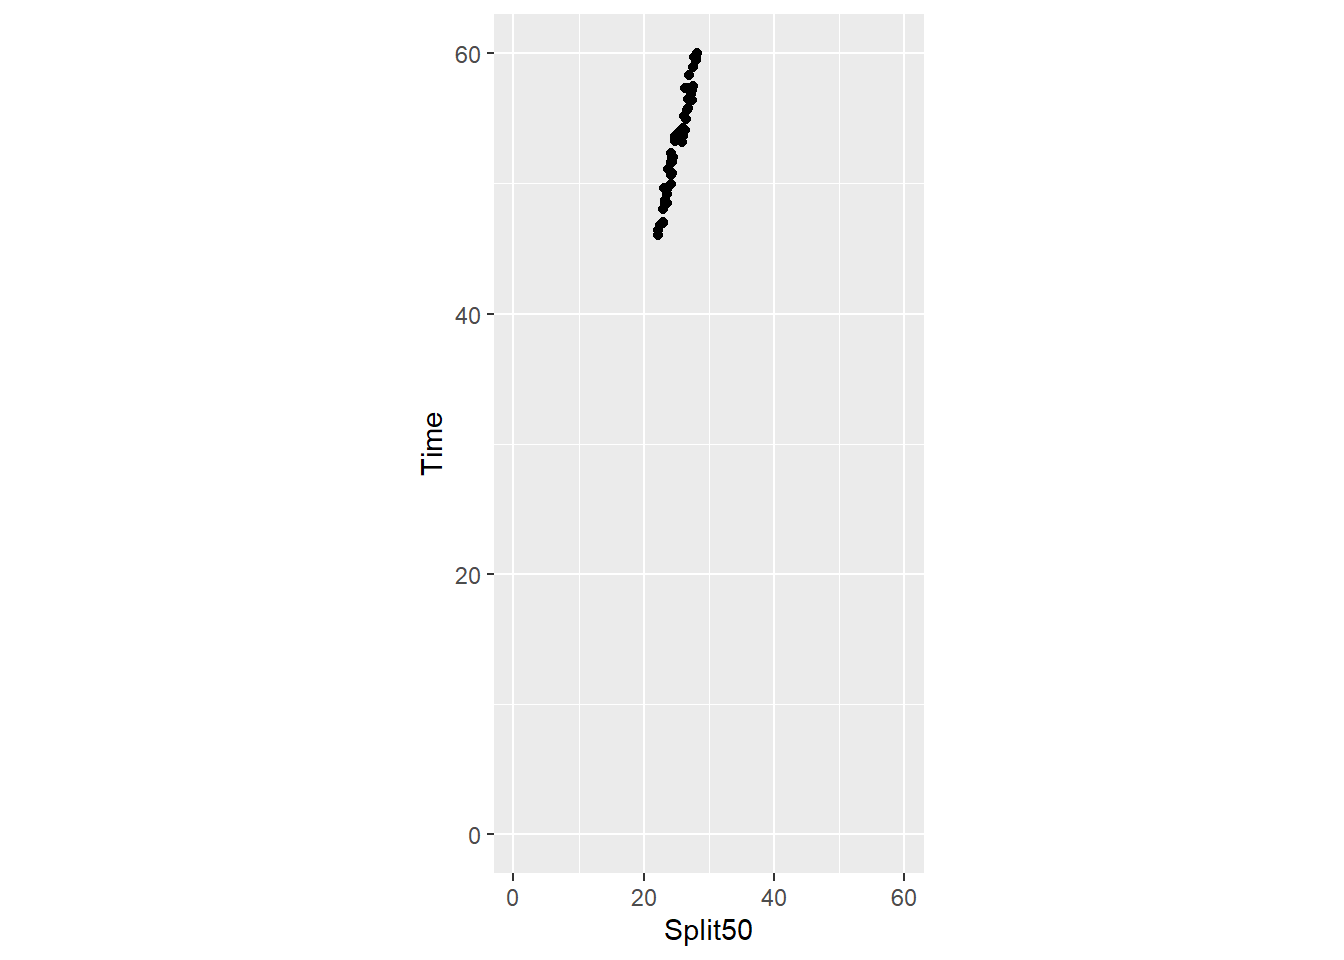
\includegraphics{01_gcds_homework_01_files/figure-latex/unnamed-chunk-7-1.pdf}

\begin{Shaded}
\begin{Highlighting}[]
\NormalTok{mtcars }\SpecialCharTok{\%\textgreater{}\%}
\NormalTok{  dplyr}\SpecialCharTok{::}\FunctionTok{mutate}\NormalTok{(}\AttributeTok{cyl =} \FunctionTok{as.factor}\NormalTok{(cyl)) }\SpecialCharTok{\%\textgreater{}\%}  \CommentTok{\# changing cylinder var to a factor }
  \FunctionTok{ggplot}\NormalTok{(., }\FunctionTok{aes}\NormalTok{(}\AttributeTok{x =}\NormalTok{ wt,                    }\CommentTok{\# x variable}
                \AttributeTok{y =}\NormalTok{ mpg)) }\SpecialCharTok{+}                \CommentTok{\# y variable}
  \FunctionTok{geom\_point}\NormalTok{(}\FunctionTok{aes}\NormalTok{(}\AttributeTok{color =}\NormalTok{ cyl)) }\SpecialCharTok{+}           \CommentTok{\# make the point colors = cyl variable}
  \FunctionTok{geom\_smooth}\NormalTok{(}\AttributeTok{method =} \StringTok{\textquotesingle{}lm\textquotesingle{}}\NormalTok{, }
              \AttributeTok{se =}\NormalTok{ F,}
              \AttributeTok{fullrange =}\NormalTok{ T) }\SpecialCharTok{+}
  \FunctionTok{facet\_wrap}\NormalTok{(}\StringTok{"cyl"}\NormalTok{)                        }\CommentTok{\# create facet for each cylinder}
\end{Highlighting}
\end{Shaded}

\begin{verbatim}
## `geom_smooth()` using formula 'y ~ x'
\end{verbatim}


\includegraphics{01_gcds_homework_01_files/figure-latex/unnamed-chunk-8-1.pdf}

\end{document}
